
\section{Results and Analysis}
Figure~\ref{fig:retention} shows retention versus access speed. FeRAM offers long retention but higher latency.

\begin{figure}[!t]
\centering
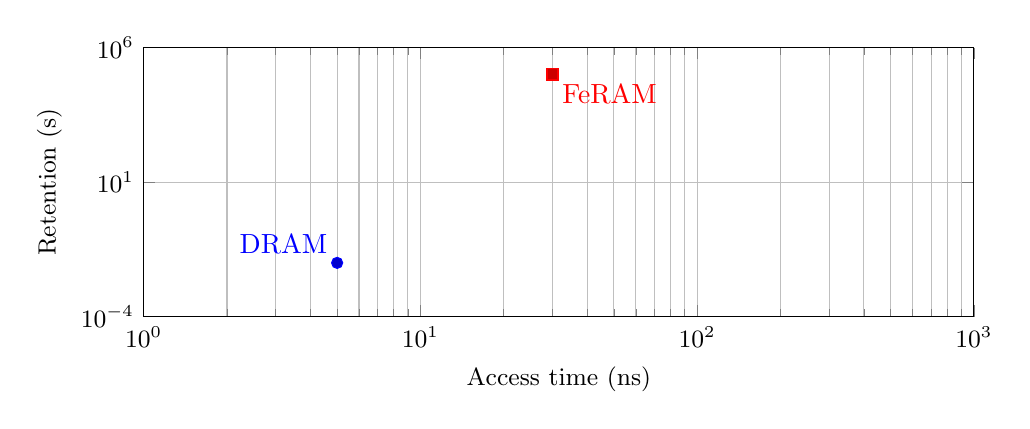
\begin{tikzpicture}
\begin{loglogaxis}[
  width=\linewidth, height=5cm,
  xlabel={Access time (ns)}, ylabel={Retention (s)},
  xmin=1e0, xmax=1e3, ymin=1e-4, ymax=1e6,
  grid=both, label style={font=\small}, tick label style={font=\small}
]
\addplot+[only marks,mark=*,mark size=2pt] coordinates {(5,1e-2)} node[above left]{DRAM};
\addplot+[only marks,mark=square*,mark size=2pt] coordinates {(30,1e5)} node[below right]{FeRAM};
\end{loglogaxis}
\end{tikzpicture}
\caption{Representative retention vs. access time.}
\label{fig:retention}
\end{figure}
